\begin{figure}[htbp]
    \centering
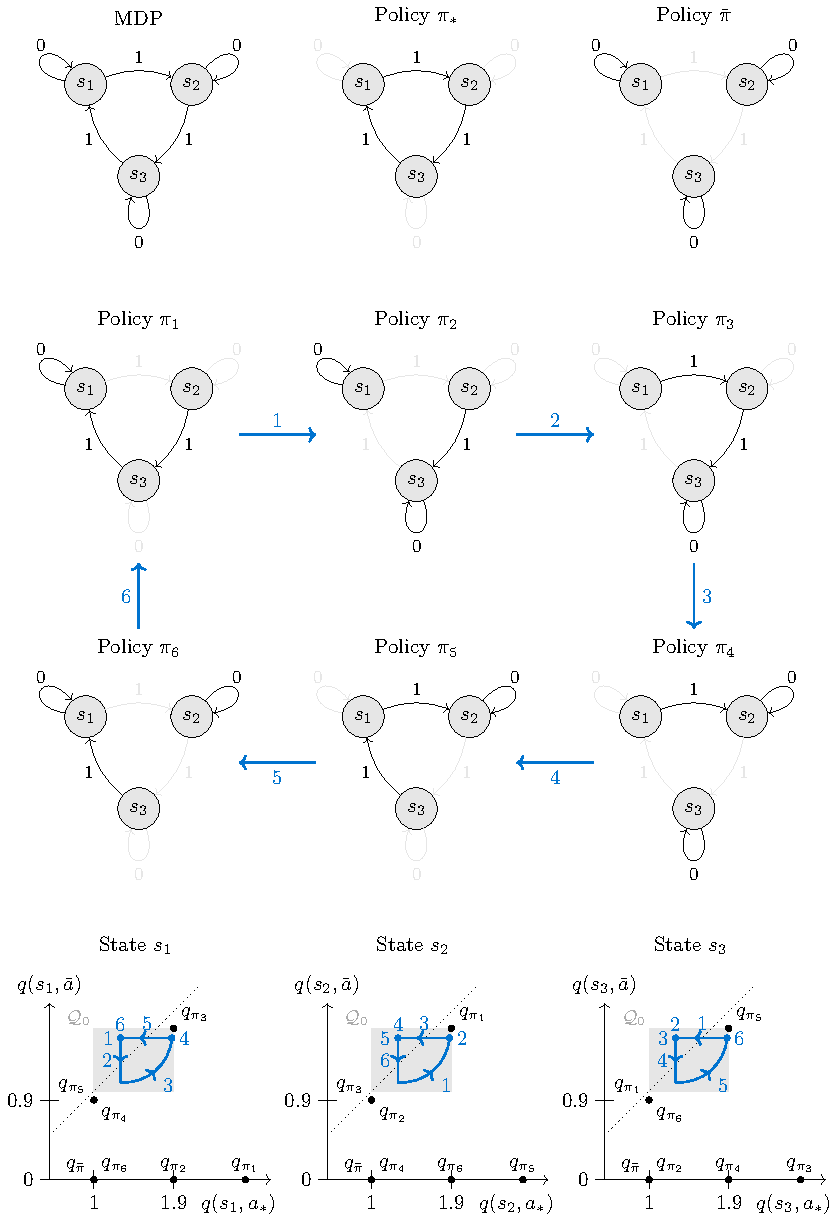
\includegraphics[width=0.95\textwidth]{figures/explain-loop-fig.pdf}
%     \pgfmathsetmacro{\shei}{0.9*1.73}
%     \pgfmathsetmacro{\swid}{0.9*2}
%     \pgfmathsetmacro{\lwid}{0.8}
    
%     \begin{subfigure}[b]{0.33\textwidth}
%         \centering
%         \begin{tikzpicture}[
%             scale=1, auto, node distance=2cm, 
%             every edge/.style={draw, <-, font=\small},
%             state/.style={circle, fill=mylightgrey, draw=black, text=black}
%         ]
%             \node at (\swid/2,\shei) [above, font=\normalsize, color=black, yshift=25pt] {MDP};
            
%             % Nodes
%             \node[state] (s1) at (0,\shei) {$s_1$};
%             \node[state] (s2) at (\swid,\shei) {$s_2$};
%             \node[state] (s3) at (\swid/2,0) {$s_3$};
%             % Edges
%             \path[->]
%                 (s1) edge[out=130, in=170, loop, looseness=8] node[pos=0.5, above] {$0$} (s1)
%                 (s2) edge[bend right=20] node[pos=0.5, above] {$1$} (s1)

%                 (s2) edge[out=10, in=50, loop, looseness=8] node[pos=0.5, above] {$0$} (s2)
%                 (s3) edge[bend right=20] node[pos=0.7, xshift=3, below] {$1$} (s2)
                
%                 (s3) edge[out=250, in=290, loop, looseness=8] node[pos=0.5, below] {$0$} (s3)
%                 (s1) edge[bend right=20] node[pos=0.3, xshift=-3, below] {$1$} (s3);
%         \end{tikzpicture}
%         % \caption{MDP}
%         \label{fig: off-policy MDP}
%     \end{subfigure}%
%     \hfill
%     \begin{subfigure}[b]{0.33\textwidth}
%         \centering
%         \begin{tikzpicture}[
%             scale=1, auto, node distance=2cm, 
%             every edge/.style={draw, <-, font=\small},
%             state/.style={circle, fill=mylightgrey, draw=black, text=black}
%         ]
%             \node at (\swid/2,\shei) [above, font=\normalsize, color=black, yshift=25pt] {Policy $\pi_*$};
        
%             % Nodes
%             \node[state] (s1) at (0,\shei) {$s_1$};
%             \node[state] (s2) at (\swid,\shei) {$s_2$};
%             \node[state] (s3) at (\swid/2,0) {$s_3$};
%             % Edges
%             \path[->]
%                 (s1) edge[out=130, in=170, loop, looseness=8, draw=mylightgrey] node[pos=0.5, above, text=mylightgrey] {$0$} (s1)
%                 (s2) edge[bend right=20] node[pos=0.5, above] {$1$} (s1)

%                 (s2) edge[out=10, in=50, loop, looseness=8, draw=mylightgrey] node[pos=0.5, above, text=mylightgrey] {$0$} (s2)
%                 (s3) edge[bend right=20] node[pos=0.7, xshift=3, below] {$1$} (s2)
                
%                 (s3) edge[out=250, in=290, loop, looseness=8, draw=mylightgrey] node[pos=0.5, below, text=mylightgrey] {$0$} (s3)
%                 (s1) edge[bend right=20] node[pos=0.3, xshift=-3, below] {$1$} (s3);
%         \end{tikzpicture}
%         % \caption{Policy $\best{\pol}$}
%     \end{subfigure}%
%     \hfill
%     \begin{subfigure}[b]{0.33\textwidth}
%         \centering
%         \begin{tikzpicture}[
%             scale=1, auto, node distance=2cm, 
%             every edge/.style={draw, <-, font=\small},
%             state/.style={circle, fill=mylightgrey, draw=black, text=black}
%         ]

%             \node at (\swid/2,\shei) [above, font=\normalsize, color=black, yshift=25pt] {Policy $\bar \pi$};
        
%             % Nodes
%             \node[state] (s1) at (0,\shei) {$s_1$};
%             \node[state] (s2) at (\swid,\shei) {$s_2$};
%             \node[state] (s3) at (\swid/2,0) {$s_3$};
%             % Edges
%             \path[->]
%                 (s1) edge[out=130, in=170, loop, looseness=8] node[pos=0.5, above] {$0$} (s1)
%                 (s2) edge[bend right=20, draw=mylightgrey] node[pos=0.5, above, text=mylightgrey] {$1$} (s1)

%                 (s2) edge[out=10, in=50, loop, looseness=8] node[pos=0.5, above] {$0$} (s2)
%                 (s3) edge[bend right=20, draw=mylightgrey] node[pos=0.7, xshift=3, below, text=mylightgrey] {$1$} (s2)
                
%                 (s3) edge[out=250, in=290, loop, looseness=8] node[pos=0.5, below] {$0$} (s3)
%                 (s1) edge[bend right=20, draw=mylightgrey] node[pos=0.3, xshift=-3, below, text=mylightgrey] {$1$} (s3);
%         \end{tikzpicture}
%         % \caption{Policy $\worst{\pol}$}
%     \end{subfigure}
   
%     \vfill
%     \vspace{0.8cm}

%     \begin{subfigure}[b]{0.33\textwidth}
%         \centering
%         \begin{tikzpicture}[
%             scale=1, auto, node distance=2cm, 
%             every edge/.style={draw, <-, font=\small},
%             state/.style={circle, fill=mylightgrey, draw=black, text=black}
%         ]
%             \node at (\swid/2,\shei) [above, font=\normalsize, color=black, yshift=25pt] {Policy $\pi_1$};

%             % Nodes
%             \node[state] (s1) at (0,\shei) {$s_1$};
%             \node[state] (s2) at (\swid,\shei) {$s_2$};
%             \node[state] (s3) at (\swid/2,0) {$s_3$};
%             % Edges
%             \path[->]
%                 (s1) edge[out=130, in=170, loop, looseness=8] node[pos=0.5, above] {$0$} (s1)
%                 (s2) edge[bend right=20, draw=mylightgrey] node[pos=0.5, above, text=mylightgrey] {$1$} (s1)

%                 (s2) edge[out=10, in=50, loop, looseness=8, draw=mylightgrey] node[pos=0.5, above, text=mylightgrey] {$0$} (s2)
%                 (s3) edge[bend right=20] node[pos=0.7, xshift=3, below] {$1$} (s2)
                
%                 (s3) edge[out=250, in=290, loop, looseness=8, draw=mylightgrey] node[pos=0.5, below, text=mylightgrey] {$0$} (s3)
%                 (s1) edge[bend right=20] node[pos=0.3, xshift=-3, below] {$1$} (s3);
% %            \draw[->,thick,red] (\swid+1,\shei/2) -- (\swid+2,\shei/2);    
%             % Cycle arrow: \pol_1 \to \pol_2.
%             \draw[overlay, ->, CambridgeCoreBlue, line width=\lwid pt]
%                 ({\swid+0.8},{\shei/2}) -- node[pos=0.5, above] {$1$} ({\swid+2.1},{\shei/2});
%             \draw[overlay, <-, CambridgeCoreBlue, line width=\lwid pt]
%                 ({\swid/2},{-1.4}) -- node[pos=0.5, left] {$6$} ({\swid/2},{-2.5});
%             % \draw[overlay, <-, CambridgeCoreBlue, line width=\lwid pt] 
%             %     (0,{-0.7}) 
%             %     to[out=225, in=135]
%             %     node[pos=0.5, left] {$6$} 
%             %     (0,{-2.7});
%         \end{tikzpicture}
%         % \caption{Policy $\pol_1$}
%     \end{subfigure}%
%     \hfill
%     \begin{subfigure}[b]{0.33\textwidth}
%         \centering
%         \begin{tikzpicture}[
%             scale=1, auto, node distance=2cm, 
%             every edge/.style={draw, <-, font=\small},
%             state/.style={circle, fill=mylightgrey, draw=black, text=black}
%         ]

%             \node at (\swid/2,\shei) [above, font=\normalsize, color=black, yshift=25pt] {Policy $\pi_2$};
        
%             % Nodes
%             \node[state] (s1) at (0,\shei) {$s_1$};
%             \node[state] (s2) at (\swid,\shei) {$s_2$};
%             \node[state] (s3) at (\swid/2,0) {$s_3$};
%             % Edges
%             \path[->]
%                 (s1) edge[out=130, in=170, loop, looseness=8] node[pos=0.5, above] {$0$} (s1)
%                 (s2) edge[bend right=20, draw=mylightgrey] node[pos=0.5, above, text=mylightgrey] {$1$} (s1)

%                 (s2) edge[out=10, in=50, loop, looseness=8, draw=mylightgrey] node[pos=0.5, above, text=mylightgrey] {$0$} (s2)
%                 (s3) edge[bend right=20] node[pos=0.7, xshift=3, below] {$1$} (s2)
                
%                 (s3) edge[out=250, in=290, loop, looseness=8] node[pos=0.5, below] {$0$} (s3)
%                 (s1) edge[bend right=20, draw=mylightgrey] node[pos=0.3, xshift=-3, below, text=mylightgrey] {$1$} (s3);
% %                            \draw[->,thick,red] (\swid+1,\shei/2) -- (\swid+2,\shei/2);    
%             % Cycle arrow: \pol_2 \to \pol_3.
%             % \draw[overlay, ->, CambridgeCoreBlue, line width=\lwid pt]
%             % ({\swid+0.8},{\shei/2}) -- node[pos=0.5, above] {$2$}  ({\swid+2.1},{\shei/2});
%         \end{tikzpicture}
%         % \caption{Policy $\pol_2$}
%     \end{subfigure}%
%     \hfill
%     \begin{subfigure}[b]{0.33\textwidth}
%         \centering
%         \begin{tikzpicture}[
%             scale=1, auto, node distance=2cm, 
%             every edge/.style={draw, <-, font=\small},
%             state/.style={circle, fill=mylightgrey, draw=black, text=black}
%         ]
%             \node at (\swid/2,\shei) [above, font=\normalsize, color=black, yshift=25pt] {Policy $\pi_3$};
        
%             % Nodes
%             \node[state] (s1) at (0,\shei) {$s_1$};
%             \node[state] (s2) at (\swid,\shei) {$s_2$};
%             \node[state] (s3) at (\swid/2,0) {$s_3$};
%             % Edges
%             \path[->]
%                 (s1) edge[out=130, in=170, loop, looseness=8, draw=mylightgrey] node[pos=0.5, above, text=mylightgrey] {$0$} (s1)
%                 (s2) edge[bend right=20] node[pos=0.5, above] {$1$} (s1)

%                 (s2) edge[out=10, in=50, loop, looseness=8, draw=mylightgrey] node[pos=0.5, above, text=mylightgrey] {$0$} (s2)
%                 (s3) edge[bend right=20] node[pos=0.7, xshift=3, below] {$1$} (s2)
                
%                 (s3) edge[out=250, in=290, loop, looseness=8] node[pos=0.5, below] {$0$} (s3)
%                 (s1) edge[bend right=20, draw=mylightgrey] node[pos=0.3, xshift=-3, below, text=mylightgrey] {$1$} (s3);
% %                            \draw[->,thick,red] (\swid+1,\shei/2) -- (\swid+1,\shei/2-4);
%             % Cycle arrow: \pol_3 \to \pol_4, routed outside the right edge
%             % so it does not cross the captions.
%             % \draw[overlay, ->, >=stealth, CambridgeCoreBlue, line width=1.7pt, shorten >=2pt]
%             %     ({\swid-0.1},{-0.10})
%             %         .. controls ({\swid+1.5},{-0.75}) and ({\swid+1.65},{-2.55}) ..
%             %     ({\swid-0.1},{-2.9});
%                 \draw[overlay, ->, CambridgeCoreBlue, line width=\lwid pt] 
%                 % ({\swid},{-0.7}) 
%                 % to[out=-45, in=45] 
%                 % node[pos=0.5, right] {$3$} 
%                 % ({\swid},{-2.7});
%                 ({\swid/2},{-1.4}) -- node[pos=0.5, right] {$3$} ({\swid/2},{-2.5});
                
%                 % ({\swid+0.45},{-0.10})
%                 %     .. controls ({\swid+1.65},{-0.75}) and ({\swid+1.65},{-2.55}) ..
%                 % ({\swid+0.95},{-3.25});

%                 \draw[overlay, <-, CambridgeCoreBlue, line width=\lwid pt]
%                 ({-0.8},{\shei/2}) -- node[pos=0.5, above] {$2$}  ({-2.1},{\shei/2});
%         \end{tikzpicture}
%         % \caption{Policy $\pol_3$}
%     \end{subfigure}
   
%     \vfill
%     \vspace{1.2cm}

%     \begin{subfigure}[b]{0.33\textwidth}
%         \centering
%         \begin{tikzpicture}[
%             scale=1, auto, node distance=2cm, 
%             every edge/.style={draw, <-, font=\small},
%             state/.style={circle, fill=mylightgrey, draw=black, text=black}
%         ]

%             \node at (\swid/2,\shei) [above, font=\normalsize, color=black, yshift=25pt] {Policy $\pi_6$};
        
%             % Nodes
%             \node[state] (s1) at (0,\shei) {$s_1$};
%             \node[state] (s2) at (\swid,\shei) {$s_2$};
%             \node[state] (s3) at (\swid/2,0) {$s_3$};
%             % Edges
%             \path[->]
%                 (s1) edge[out=130, in=170, loop, looseness=8] node[pos=0.5, above] {$0$} (s1)
%                 (s2) edge[bend right=20, draw=mylightgrey] node[pos=0.5, above, text=mylightgrey] {$1$} (s1)

%                 (s2) edge[out=10, in=50, loop, looseness=8] node[pos=0.5, above] {$0$} (s2)
%                 (s3) edge[bend right=20, draw=mylightgrey] node[pos=0.7, xshift=3, below, text=mylightgrey] {$1$} (s2)
                
%                 (s3) edge[out=250, in=290, loop, looseness=8, draw=mylightgrey] node[pos=0.5, below, text=mylightgrey] {$0$} (s3)
%                 (s1) edge[bend right=20] node[pos=0.3, xshift=-3, below] {$1$} (s3);
%             % Cycle arrow: \pol_6 \to \pol_1, routed outside the left edge
%             % so it does not cross the captions.
%             % \draw[overlay, ->, >=stealth, CambridgeCoreBlue, line width=1.7pt, shorten >=2pt]
%             %     ({-0.75},{\shei+0.10})
%             %         .. controls ({-1.65},{\shei+0.75}) and ({-1.65},{\shei+2.55}) ..
%             %     ({-0.95},{\shei+3.25});
%             % \draw[overlay, ->, CambridgeCoreBlue, line width=\lwid pt] 
%             %     (0,{\shei+0.10}) 
%             %     to[out=135, in=225]
%             %     node[pos=0.5, left] {$6$} 
%             %     (0,{\shei+3.25});
%             \draw[overlay, <-, CambridgeCoreBlue, line width=\lwid pt]
%                 ({\swid+0.8},{\shei/2}) -- node[pos=0.5, below] {$5$} ({\swid+2.1},{\shei/2});
%         \end{tikzpicture}
%         % \caption{Policy $\pol_6$}
%     \end{subfigure}
%    \hfill
%     \begin{subfigure}[b]{0.33\textwidth}
%         \centering
%         \begin{tikzpicture}[
%             scale=1, auto, node distance=2cm, 
%             every edge/.style={draw, <-, font=\small},
%             state/.style={circle, fill=mylightgrey, draw=black, text=black}
%         ]
%             \node at (\swid/2,\shei) [above, font=\normalsize, color=black, yshift=25pt] {Policy $\pi_5$};
        
%             % Nodes
%             \node[state] (s1) at (0,\shei) {$s_1$};
%             \node[state] (s2) at (\swid,\shei) {$s_2$};
%             \node[state] (s3) at (\swid/2,0) {$s_3$};
%             % Edges
%             \path[->]
%                 (s1) edge[out=130, in=170, loop, looseness=8, draw=mylightgrey] node[pos=0.5, above, text=mylightgrey] {$0$} (s1)
%                 (s2) edge[bend right=20] node[pos=0.5, above] {$1$} (s1)

%                 (s2) edge[out=10, in=50, loop, looseness=8] node[pos=0.5, above] {$0$} (s2)
%                 (s3) edge[bend right=20, draw=mylightgrey] node[pos=0.7, xshift=3, below, text=mylightgrey] {$1$} (s2)
                
%                 (s3) edge[out=250, in=290, loop, looseness=8, draw=mylightgrey] node[pos=0.5, below, text=mylightgrey] {$0$} (s3)
%                 (s1) edge[bend right=20] node[pos=0.3, xshift=-3, below] {$1$} (s3);
%             % Cycle arrow: \pol_5 \to \pol_6.
%             % \draw[overlay, ->, CambridgeCoreBlue, line width=\lwid pt]
%             %     ({-0.55},{\shei/2}) -- node[pos=0.5, below] {$5$} ({-2.25},{\shei/2});
%         \end{tikzpicture}
%         % \caption{Policy $\pol_5$}
%     \end{subfigure}%
%     \hfill
%  \begin{subfigure}[b]{0.33\textwidth}
%         \centering
%         \begin{tikzpicture}[
%             scale=1, auto, node distance=2cm, 
%             every edge/.style={draw, <-, font=\small},
%             state/.style={circle, fill=mylightgrey, draw=black, text=black}
%         ]
%             \node at (\swid/2,\shei) [above, font=\normalsize, color=black, yshift=25pt] {Policy $\pi_4$};
        
%             % Nodes
%             \node[state] (s1) at (0,\shei) {$s_1$};
%             \node[state] (s2) at (\swid,\shei) {$s_2$};
%             \node[state] (s3) at (\swid/2,0) {$s_3$};
%             % Edges
%             \path[->]
%                 (s1) edge[out=130, in=170, loop, looseness=8, draw=mylightgrey] node[pos=0.5, above, text=mylightgrey] {$0$} (s1)
%                 (s2) edge[bend right=20] node[pos=0.5, above] {$1$} (s1)

%                 (s2) edge[out=10, in=50, loop, looseness=8] node[pos=0.5, above] {$0$} (s2)
%                 (s3) edge[bend right=20, draw=mylightgrey] node[pos=0.7, xshift=3, below, text=mylightgrey] {$1$} (s2)
                
%                 (s3) edge[out=250, in=290, loop, looseness=8] node[pos=0.5, below] {$0$} (s3)
%                 (s1) edge[bend right=20, draw=mylightgrey] node[pos=0.3, xshift=-3, below, text=mylightgrey] {$1$} (s3);
%             % Cycle arrow: \pol_4 \to \pol_5.
%             \draw[overlay, ->, CambridgeCoreBlue, line width=\lwid pt]
%                 ({-0.8},{\shei/2}) -- node[pos=0.5, below] {$4$}  ({-2.1},{\shei/2});
%         \end{tikzpicture}
%         % \caption{Policy $\pol_4$}
%     \end{subfigure}%
    
%     \vspace{0.8cm}
   
%    \begin{subfigure}[b]{.32\textwidth}
%         \centering
%         \normalsize{State $s_1$}
        
%         {\begin{tikzpicture}[scale=1.5]
%             % Draw the grid and axes
%             % \draw[step=0.5cm,very thin,mylightgrey] (0,0) grid (3,3);
%             \draw[thin,->] (.5,0) -- (3,0) node[below left, xshift=6pt, yshift=-3pt] {$q(s_1,\best{a})$};
%             \draw[thin,->] (0.5,0) -- (0.5,2) node[above] {$q(s_1,\worst{a})$};
%             % \draw[thick,->] (0,0) -- (3.2,0) node[right] {\shortstack{$\best{a}$ \\ $\pol_1, \pol_5, \pol_6$}};
%             % \draw[thick,->] (0,0) -- (0,2.2) node[above] {\shortstack{$\worst{a}$ \\ $\pol_2, \pol_3, \pol_4$}};

%             \node at (1, 1.71) [above left, font=\small, color=mygrey, xshift=2pt, yshift=-2pt] {$\mathcal Q_0$};

%             % Draw the grey square from (1,1) to (2,2)
%             \filldraw[fill=mylightgrey, draw=none] (1,1) rectangle (1.9,1.71);
            
%             % Draw the line y = x
%             \draw[dotted, black] (0.5,0.5) -- (2.2,2.2);

%             % Add the points with associated text
%             \filldraw (2.71,0) circle (1pt) node[above] {$q_{\pol_1}$};
%             \filldraw (1.9,1.71) circle (1pt) node[above right] {$q_{\pol_3}$};
%             \filldraw (1.9,0) circle (1pt) node[above] {$q_{\pol_2}$};
%             \filldraw (1,0.9) circle (1pt) node[above left] {$q_{\pol_5}$};
%             \filldraw (1,0.9) circle (1pt) node[below right] {$q_{\pol_4}$};
%             \filldraw (1,0) circle (1pt) node[above right] {$q_{\pol_6}$};
%             \filldraw (1,0) circle (1pt) node[above left] {$q_{\worst{\pol}}$};
            
%             % Add labels to the axes
%             % \draw (0,0.1) -- (0,-0.1) node[left, font=\normalsize, xshift=-4.5pt, yshift=-6.5pt] {0};
%             %\draw (0,0.1) -- (0,-0.1) node[below, font=\normalsize] {0};
% %            \draw (-0.1,0) -- (0.1,0) node[font=\normalsize] {};
%             \foreach \x in {1,1.9}
%                 \draw (\x,0.1) -- (\x,-0.1) node[below, font=\normalsize] {\x};
%             \foreach \y in {0,0.9}
%                 \draw (.5+0.1,\y) -- (.5-0.1,\y) node[left, font=\normalsize] {\y};

%             % Add the red arrows
%             \draw[middle arrow=0.65, CambridgeCoreBlue, line width=\lwid pt] (1.9, 1.6) -- (1.3, 1.6) node[midway, above, sloped, font=\normalsize] {$5$};
%             \draw[middle arrow=0.55, CambridgeCoreBlue, line width=\lwid pt] (1.3, 1.6) -- (1.3, 1.1) node[midway, left, font=\normalsize] {$2$};
%             % \draw[middle arrow=0.5, CambridgeCoreBlue, thick] (1.3, 1.1) -- (1.9, 1.7) node[midway, below, sloped, font=\normalsize] {3};

%             \draw[middle arrow=0.5, CambridgeCoreBlue, line width=\lwid pt] 
%             (1.3,1.1) to[bend right=45] 
%             node[midway, below right, font=\normalsize] {$3$}
%             (1.88,1.6);

%             % \draw[thick, CambridgeCoreBlue] (1.45, 1.7) -- (1.45, 1.25);

%             \filldraw[fill=CambridgeCoreBlue, draw=CambridgeCoreBlue] (1.3,1.6) circle (1pt) node[left, text=CambridgeCoreBlue, font=\normalsize] {$1$};
%             \filldraw[fill=CambridgeCoreBlue, draw=CambridgeCoreBlue] (1.3,1.6) circle (0pt) node[above, text=CambridgeCoreBlue, font=\normalsize] {$6$};
%             \filldraw[fill=CambridgeCoreBlue, draw=CambridgeCoreBlue] (1.88,1.6) circle (1pt) node[right, text=CambridgeCoreBlue, font=\normalsize] {$4$};
            
%         \end{tikzpicture}}
%         % \caption{State $s_1$}
%         \end{subfigure}
%            \begin{subfigure}[b]{.32\textwidth}
%         \centering
%         \normalsize{State $s_2$}
        
%         {\begin{tikzpicture}[scale=1.5]
%             % Draw the grid and axes
%             % \draw[step=0.5cm,very thin,mylightgrey] (0,0) grid (3,3);
%             \draw[thin,->] (.5,0) -- (3,0) node[below left, xshift=6pt, yshift=-3pt] {$q(s_2,\best{a})$};
%             \draw[thin,->] (0.5,0) -- (0.5,2) node[above] {$q(s_2,\worst{a})$};
%             % \draw[thick,->] (0,0) -- (3.2,0) node[right] {\shortstack{$\best{a}$ \\ $\pol_1, \pol_5, \pol_6$}};
%             % \draw[thick,->] (0,0) -- (0,2.2) node[above] {\shortstack{$\worst{a}$ \\ $\pol_2, \pol_3, \pol_4$}};

%             % \node at (1.6, 2.2) [above, font=\normalsize, color=black] {State $s_1$};

%             \node at (1, 1.71) [above left, font=\small, color=mygrey, xshift=2pt, yshift=-2pt] {$\mathcal Q_0$};

%             % Draw the grey square from (1,1) to (2,2)
%             \filldraw[fill=mylightgrey, draw=none] (1,1) rectangle (1.9,1.71);
            
%             % Draw the line y = x
%             \draw[dotted, black] (0.5,0.5) -- (2.2,2.2);

%             % Add the points with associated text
%             \filldraw (2.71,0) circle (1pt) node[above] {$q_{\pol_5}$};
%             \filldraw (1.9,1.71) circle (1pt) node[above right] {$q_{\pol_1}$};
%             \filldraw (1.9,0) circle (1pt) node[above] {$q_{\pol_6}$};
%             \filldraw (1,0.9) circle (1pt) node[above left] {$q_{\pol_3}$};
%             \filldraw (1,0.9) circle (1pt) node[below right] {$q_{\pol_2}$};
%             \filldraw (1,0) circle (1pt) node[above right] {$q_{\pol_4}$};
%             \filldraw (1,0) circle (1pt) node[above left] {$q_{\worst{\pol}}$};
            
%             % Add labels to the axes
%             % \draw (0,0.1) -- (0,-0.1) node[left, font=\normalsize, xshift=-4.5pt, yshift=-6.5pt] {0};
%             %\draw (0,0.1) -- (0,-0.1) node[below, font=\normalsize] {0};
% %            \draw (-0.1,0) -- (0.1,0) node[font=\normalsize] {};
%             \foreach \x in {1,1.9}
%                 \draw (\x,0.1) -- (\x,-0.1) node[below, font=\normalsize] {\x};
%             \foreach \y in {0,0.9}
%                 \draw (.5+0.1,\y) -- (.5-0.1,\y) node[left, font=\normalsize] {\y};

%             % Add the red arrows
%             \draw[middle arrow=0.65, CambridgeCoreBlue, line width=\lwid pt] (1.9, 1.6) -- (1.3, 1.6) node[midway, above, sloped, font=\normalsize] {$3$};
%             \draw[middle arrow=0.55, CambridgeCoreBlue, line width=\lwid pt] (1.3, 1.6) -- (1.3, 1.1) node[midway, left, font=\normalsize] {$6$};
%             % \draw[middle arrow=0.5, CambridgeCoreBlue, thick] (1.3, 1.1) -- (1.9, 1.7) node[midway, below, sloped, font=\normalsize] {3};

%             \draw[middle arrow=0.5, CambridgeCoreBlue, line width=\lwid pt] 
%             (1.3,1.1) to[bend right=45] 
%             node[midway, below right, font=\normalsize] {$1$}
%             (1.88,1.6);

%             % \draw[thick, CambridgeCoreBlue] (1.45, 1.7) -- (1.45, 1.25);

%             \filldraw[fill=CambridgeCoreBlue, draw=CambridgeCoreBlue] (1.3,1.6) circle (1pt) node[left, text=CambridgeCoreBlue, font=\normalsize] {$5$};
%             \filldraw[fill=CambridgeCoreBlue, draw=CambridgeCoreBlue] (1.3,1.6) circle (0pt) node[above, text=CambridgeCoreBlue, font=\normalsize] {$4$};
%             \filldraw[fill=CambridgeCoreBlue, draw=CambridgeCoreBlue] (1.88,1.6) circle (1pt) node[right, text=CambridgeCoreBlue, font=\normalsize] {$2$};
            
%         \end{tikzpicture}}
%         % \caption{State $s_3$}
%         \end{subfigure}
%            \begin{subfigure}[b]{.32\textwidth}
%         \centering
%         \normalsize{State $s_3$}
        
%         {\begin{tikzpicture}[scale=1.5]
%             % Draw the grid and axes
%             % \draw[step=0.5cm,very thin,mylightgrey] (0,0) grid (3,3);
%             \draw[thin,->] (.5,0) -- (3,0) node[below left, xshift=6pt, yshift=-3pt] {$q(s_3,\best{a})$};
%             \draw[thin,->] (0.5,0) -- (0.5,2) node[above] {$q(s_3,\worst{a})$};
%             % \draw[thick,->] (0,0) -- (3.2,0) node[right] {\shortstack{$\best{a}$ \\ $\pol_1, \pol_5, \pol_6$}};
%             % \draw[thick,->] (0,0) -- (0,2.2) node[above] {\shortstack{$\worst{a}$ \\ $\pol_2, \pol_3, \pol_4$}};

%             % \node at (1.6, 2.2) [above, font=\normalsize, color=black] {State $s_1$};

%             \node at (1, 1.71) [above left, font=\small, color=mygrey, xshift=2pt, yshift=-2pt] {$\mathcal Q_0$};

%             % Draw the grey square from (1,1) to (2,2)
%             \filldraw[fill=mylightgrey, draw=none] (1,1) rectangle (1.9,1.71);
            
%             % Draw the line y = x
%             \draw[dotted, black] (0.5,0.5) -- (2.2,2.2);

%             % Add the points with associated text
%             \filldraw (2.71,0) circle (1pt) node[above] {$q_{\pol_3}$};
%             \filldraw (1.9,1.71) circle (1pt) node[above right] {$q_{\pol_5}$};
%             \filldraw (1.9,0) circle (1pt) node[above] {$q_{\pol_4}$};
%             \filldraw (1,0.9) circle (1pt) node[above left] {$q_{\pol_1}$};
%             \filldraw (1,0.9) circle (1pt) node[below right] {$q_{\pol_6}$};
%             \filldraw (1,0) circle (1pt) node[above right] {$q_{\pol_2}$};
%             \filldraw (1,0) circle (1pt) node[above left] {$q_{\worst{\pol}}$};
            
%             % Add labels to the axes
%             % \draw (0,0.1) -- (0,-0.1) node[left, font=\normalsize, xshift=-4.5pt, yshift=-6.5pt] {0};
%             %\draw (0,0.1) -- (0,-0.1) node[below, font=\normalsize] {0};
% %            \draw (-0.1,0) -- (0.1,0) node[font=\normalsize] {};
%             \foreach \x in {1,1.9}
%                 \draw (\x,0.1) -- (\x,-0.1) node[below, font=\normalsize] {\x};
%             \foreach \y in {0,0.9}
%                 \draw (.5+0.1,\y) -- (.5-0.1,\y) node[left, font=\normalsize] {\y};

%             % Add the red arrows
%             \draw[middle arrow=0.65, CambridgeCoreBlue, line width=\lwid pt] (1.9, 1.6) -- (1.3, 1.6) node[midway, above, sloped, font=\normalsize] {$1$};
%             \draw[middle arrow=0.55, CambridgeCoreBlue, line width=\lwid pt] (1.3, 1.6) -- (1.3, 1.1) node[midway, left, font=\normalsize] {$4$};
%             % \draw[middle arrow=0.5, CambridgeCoreBlue, thick] (1.3, 1.1) -- (1.9, 1.7) node[midway, below, sloped, font=\normalsize] {3};

%             \draw[middle arrow=0.5, CambridgeCoreBlue, line width=\lwid pt] 
%             (1.3,1.1) to[bend right=45] 
%             node[midway, below right, font=\normalsize] {$5$}
%             (1.88,1.6);

%             % \draw[thick, CambridgeCoreBlue] (1.45, 1.7) -- (1.45, 1.25);

%             \filldraw[fill=CambridgeCoreBlue, draw=CambridgeCoreBlue] (1.3,1.6) circle (1pt) node[left, text=CambridgeCoreBlue, font=\normalsize] {$3$};
%             \filldraw[fill=CambridgeCoreBlue, draw=CambridgeCoreBlue] (1.3,1.6) circle (0pt) node[above, text=CambridgeCoreBlue, font=\normalsize] {$2$};
%             \filldraw[fill=CambridgeCoreBlue, draw=CambridgeCoreBlue] (1.88,1.6) circle (1pt) node[right, text=CambridgeCoreBlue, font=\normalsize] {$6$};
            
%         \end{tikzpicture}}
%         % \caption{State $s_1$}
%         \end{subfigure}
    \caption{The sampling strategy described on page \pageref{pg: sampling strat 3 states} forces IV MC-O-PI to cycle indefinitely between six suboptimal policies
    % $\pol_1$, $\pol_2$, $\pol_3$, $\pol_4$, $\pol_5$ and $\pol_6$ 
    for every initial condition in $\qset_0$.
    This figure depicts the expected cycle in the policies $\{\pi_k\}_{k\ge 0}$ (middle) and in the estimates $\{q_k\}_{k\ge 0}$ (bottom).
    The "move" action correspond to $a_*$, and "stay" to $\bar a$.
    The dotted lines are the boundaries between regions, namely where $q(s,a_*) = q(s,\bar a)$.}
    % Spiral obtained for every initial condition in $\qset_0$ with the sampling strategy described on page \pageref{enum: sampling greedy initial visit}.
    % MC-O-PI cycles indefinitely between the policies $\pol_1$ through $\pol_6$ despite the update distributions with a greedy bias.}
    \label{fig: explain loop on-policy bias MDP}
    \end{figure}%
